%!TeX root = main.tex
%!encoding = UTF-8 Unicode
\chapter{Electromagnetic Emissions of Switching Transients and Measurement Principles}
\label{ch:Fundamentals}

This chapter establishes the physical and metrological basis for characterizing the electromagnetic emission behavior of power semiconductor devices.
It relates switching waveforms to their source spectra, explains how propagation paths shape system-level emissions, and distinguishes source characterization from standardized EMC compliance measurements.
Here, intrinsic emission behavior refers to the device-level switching behavior under defined operating and circuit conditions, before transfer to an external system port; it is not a property independent of the gate drive, complementary device, or circuit parasitics.
The chapter then examines errors in dynamic voltage and current measurements and derives verification criteria for the probes developed in Sections~\ref{ch:voltage} and~\ref{ch:AShunt}.
These fundamentals provide the basis for the measurement limitations and methodological developments addressed in Chapter~\ref{ch:Methods}.

%!TeX root = main.tex
%!encoding = UTF-8 Unicode
\section{EMC in Power Electronics}

Electromagnetic compatibility (EMC) describes the ability of electrical and electronic equipment to operate in an electromagnetic environment as intended without causing or experiencing unacceptable interference. 
An EMC problem generally involves three elements: a noise source, a propagation path, and a noise sink. 
The noise source generates electromagnetic disturbances, the propagation path transfers them through conducted or radiated coupling, and the sink responds to the resulting disturbance. 
\fref{fig:BlockDiagram_SourceVictim} illustrates this model with a measurement port in the propagation path.
The port can be used to measure disturbances from the source or to inject a defined disturbance for an immunity test of the sink.
\begin{figure}
	\centering\import{./figures/2_Fundamentals/}{BlockDiagram_SourceVictim.pdf_tex}
	\caption{Block diagram of EM interaction between source, propagation path, and sink.}
	\label{fig:BlockDiagram_SourceVictim}
\end{figure}

In a power-electronic converter, the switching semiconductor devices are the dominant noise sources, while the converter layout, passive components, cables, and enclosure determine the available propagation paths. 
Other circuits or sensors connected to, or located near, the converter may act as victims.
This situation is particularly relevant in electric vehicles, where high-power inverters are located close to sensitive electronic components and sensors, such as those used for safety applications and autonomous-driving systems.

\FloatBarrier

\subsection{Emission Generation}
\label{sec:Fundamental_Generation}
The fast voltage and current transients produced by switching power-semiconductor devices excite electromagnetic disturbances in the surrounding circuit.
Following the graphical approach presented by Costa~\cite{costa_graphical_2005}, the analysis starts with a periodic rectangular pulse and then introduces finite transition times, waveform asymmetry, and resonance.
Gaussian smoothing provides a theoretical reference for spectral concentration, while a simulated waveform illustrates the combined effects and the need for experimental validation.
The analysis concerns the switching-voltage spectrum at the source, rather than the emissions at a system port.

\subsubsection*{Rectangular-Pulse Spectrum}
\textbf{Isolated Pulse:} A rectangular pulse provides the simplest representation of a switching waveform and serves as the starting point for the analysis:

\begin{equation}
	s(t) = \mi{V}{DC}\cdot\text{rect}\left(\frac{t}{\text{d}\mi{T}{s}}\right), 
\end{equation}
where \mi{V}{DC} is the DC-link voltage, $\text{d}$ is the duty cycle, and \mi{T}{s} is the switching period.
Using the Fourier-transform convention with kernel $e^{-j2\pi ft}$ gives
\begin{equation}
	S(f) = \mi{V}{DC}\cdot\text{d}\mi{T}{s}\cdot\text{si}\left(\pi f\text{d}\mi{T}{s}\right),
\end{equation}
where $\text{si}(x) = \sin(x)/x$ and $\text{si}(0) = 1$.
Because the Fourier transform integrates voltage over time, $S(f)$ has units of voltage multiplied by time. It describes the continuous spectrum of one isolated pulse; voltage-valued Fourier-series coefficients arise when the pulse is repeated periodically, as described next.

\textbf{Periodic Pulse Chain:} To represent steady-state switching, the isolated pulse is repeated at the switching period by convolution with a Dirac comb, forming a periodic pulse chain (PC):
\begin{equation}
	\mi{s}{PC}(t) = s(t) * \sum_{n=-\infty}^{\infty} \delta(t-\text{n}\mi{T}{s}).
\end{equation}
With $\mi{f}{s} = 1/\mi{T}{s}$, its Fourier transform becomes
\begin{equation}
	\mi{S}{PC}(f) = \sum_{n=-\infty}^{\infty} \frac{S(\text{n}\mi{f}{s})}{\mi{T}{s}}\,\delta(f-\text{n}\mi{f}{s}).
\end{equation}
Periodic repetition thus produces discrete spectral lines at integer multiples of the switching frequency.
For harmonic order $n$, the complex Fourier-series coefficient is $S(\text{n}\mi{f}{s})/\mi{T}{s}$.
Its magnitude is given by the continuous two-sided coefficient envelope evaluated at that harmonic:
\begin{equation}
A(f) = \frac{|S(f)|}{\mi{T}{s}}.
\end{equation}


\textbf{Spectral Envelope:} Logarithmic frequency and decibel voltage scales facilitate comparison of EMC spectra spanning several orders of magnitude.
Accordingly, the two-sided coefficient envelope $A(f)$ is expressed in logarithmic form relative to a voltage reference \mi{V}{ref}:
\begin{equation}
A_\text{dB}(f) = 20\log_{10}\left(\frac{A(f)}{\mi{V}{ref}}\right).
\end{equation}
The reference $\mi{V}{ref} = \SI{1}{\micro\volt}$ gives levels in dB\textmu V.
Here, $A(f)$ denotes a two-sided Fourier-series coefficient magnitude, not a single-sided peak or RMS amplitude.
For a real waveform, the corresponding nonzero harmonic has peak amplitude $2A(n\mi{f}{s})$ and RMS amplitude $\sqrt{2}A(n\mi{f}{s})$.
This normalization must be accounted for when comparing the analytical envelope with FFT results or receiver readings.

For the rectangular pulse shown in \fref{fig:Diss_SpectrumCreation_zeroOrder}, the low-frequency asymptote is the DC coefficient $\text{d}\mi{V}{DC}$, while the high-frequency envelope decreases in proportion to $1/f$, corresponding to a \SI{-20}{dB/dec} slope in a logarithmic plot.
The intersection of these asymptotes defines the first corner frequency:
\begin{equation}
	\mi{f}{c1} = \frac{1}{\pi\text{d}\mi{T}{s}}.
\end{equation}
This corner frequency is an intersection of asymptotes, not a sharp transition in the exact si-function spectrum.

\begin{figure}[h]
	\centering
	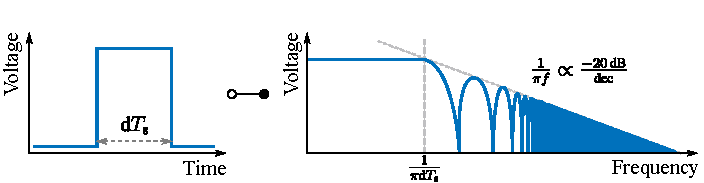
\includegraphics[scale = 1]{figures/2_Fundamentals/Diss_SpectrumCreation_zeroOrder.pdf}
	\caption{Graphical representation of the creation of the emission spectrum from a zero-order approximation of the switching transient.}
	\label{fig:Diss_SpectrumCreation_zeroOrder}
\end{figure}
\FloatBarrier


\subsubsection*{Influence of the Transition Shape}
\textbf{Equal Rise and Fall Times:} The rectangular approximation neglects the finite switching speed of real semiconductor devices.
Introducing linear transitions of equal duration \mi{t}{r} gives a trapezoidal pulse, obtained by convolving the rectangular pulse with a unit-area rectangular smoothing kernel:
\begin{equation}
	s(t) = \mi{V}{DC}\cdot\text{rect}\left(\frac{t}{\text{d}\mi{T}{s}}\right) *\frac{1}{\mi{t}{r}} \text{rect}\left(\frac{t}{\mi{t}{r}}\right).
\end{equation}
The convolution smooths the switching edges while preserving the pulse area.
Convolution in the time domain corresponds to multiplication in the frequency domain:
\begin{equation}
	S(f) = \mi{V}{DC}\cdot\text{d}\mi{T}{s}\cdot\text{si}\left(\pi f\text{d}\mi{T}{s}\right) \cdot \text{si}\left(\pi f \mi{t}{r}\right).
\end{equation}
The second si factor introduces an additional corner frequency,
\begin{equation}
	\mi{f}{c2} = \frac{1}{\pi\mi{t}{r}}.
\end{equation}
For $\mi{t}{r} \ll \text{d}\mi{T}{s}$, the envelope has three distinct regions: an approximately constant low-frequency region, a \SI{-20}{dB/dec} region, and a \SI{-40}{dB/dec} region above \mi{f}{c2}.
As illustrated in \fref{fig:Diss_SpectrumCreation_firstOrder}, the pulse duration and transition duration therefore control different parts of the envelope: the former sets the first corner, while the latter determines the onset of the additional high-frequency attenuation.

\begin{figure}[h]
	\centering
	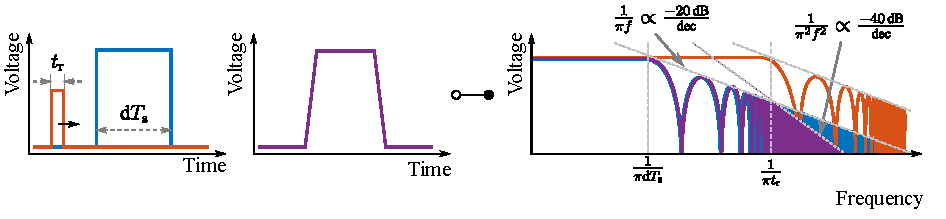
\includegraphics[scale = 1]{figures/2_Fundamentals/Diss_SpectrumCreation_firstOrder.pdf}
	\caption{Graphical representation of the creation of the emission spectrum from a first-order approximation of the switching transient.}
	\label{fig:Diss_SpectrumCreation_firstOrder}
\end{figure}

\textbf{Unequal Rise and Fall Times:}
Power-semiconductor devices generally exhibit different switching speeds during turn-on and turn-off, resulting in unequal rise and fall times.
To account for this asymmetry, the convolution-based approximation introduces separate transition-shaping terms for the rising and falling edges, as illustrated in \fref{fig:Diss_SpectrumCreation_asymTr}:
\begin{equation}
	s(t) = \mi{V}{DC} \cdot \text{rect}\left(\frac{t}{\text{d}\mi{T}{s}}\right) * \left(\mi{s}{sw,r} + \mi{s}{sw,f}\right)
\end{equation}
where \mi{s}{sw,r} and \mi{s}{sw,f} represent the respective transition-shaping terms.
In the graphical spectral approximation, the corresponding contributions are expressed as the sum of two si~functions:
\begin{equation}
	S(f) = \mi{V}{DC}\cdot\text{d}\mi{T}{s}\cdot\text{si}\left(\pi f\text{d}\mi{T}{s}\right) \cdot \left(\text{si}\left(\pi f \mi{t}{r}\right) + \text{si}\left(\pi f \mi{t}{f}\right)\right)
\end{equation}

The two transition durations introduce distinct corner frequencies, $1/(\pi\mi{t}{r})$ and $1/(\pi\mi{t}{f})$.
The longer transition begins to attenuate its spectral contribution at a lower frequency, allowing the faster edge to dominate between the two corners.
Above both corners, the asymptotic envelope decreases again at \SI{-40}{dB/dec}.

\begin{figure}[h]
	\centering
	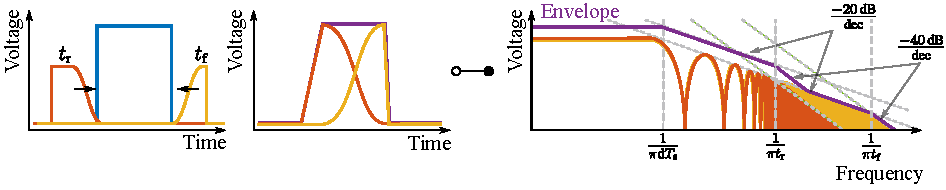
\includegraphics[scale = 1]{figures/2_Fundamentals/Diss_SpectrumCreation_asymTr.pdf}
	\caption{Switching waveform and spectral envelope for unequal rise and fall times.}
	\label{fig:Diss_SpectrumCreation_asymTr}
\end{figure}
\FloatBarrier

\textbf{Two-Slope Transitions:}
Whereas the preceding approximation distinguishes the rising and falling edges, a two-slope approximation accounts for changes in slope within an individual transition.
During turn-on, for example, the initial drain-source voltage change is influenced by the commutation-loop inductance and the current rise, while the subsequent voltage fall is governed by the gate drive and device capacitances.
This behavior is represented by convolving the rectangular pulse with the sum of two rectangular smoothing functions of different durations, as illustrated in \fref{fig:Diss_SpectrumCreation_twoTr}:
\begin{equation}
	s(t) = \mi{V}{DC} \cdot \text{rect}\left(\frac{t}{\text{d}\mi{T}{s}}\right) * \left(\frac{1}{\mi{t}{r1}} \text{rect}\left(\frac{t}{\mi{t}{r1}}\right) + \frac{1}{\mi{t}{r2}} \text{rect}\left(\frac{t}{\mi{t}{r2}}\right)\right)
\end{equation}
The corresponding frequency-domain expression is
\begin{equation}
	S(f) = \mi{V}{DC}\cdot\text{d}\mi{T}{s}\cdot\text{si}\left(\pi f\text{d}\mi{T}{s}\right) \cdot \left(\text{si}\left(\pi f \mi{t}{r1}\right) + \text{si}\left(\pi f \mi{t}{r2}\right)\right)
\end{equation}

This expression has the same mathematical form as the preceding graphical approximation, but the two durations now characterize contributions within a switching edge rather than separate rising and falling edges.

\begin{figure}[h]
	\centering
	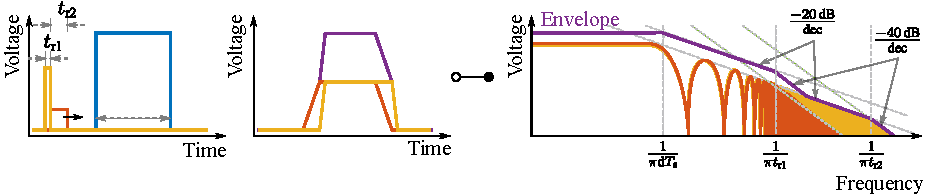
\includegraphics[scale = 1]{figures/2_Fundamentals/Diss_SpectrumCreation_twoTr.pdf}
	\caption{Switching waveform and spectral envelope for a two-slope transition approximation.}
	\label{fig:Diss_SpectrumCreation_twoTr}
\end{figure}
\FloatBarrier

\subsubsection*{Resonant Contributions}
Whereas the preceding models describe monotonic transitions, practical switching waveforms often exhibit overshoot followed by damped oscillations.
The underlying resonances arise from the interaction between the commutation-loop inductance and the output capacitance of the device in the off state.
Their excitation adds spectral contributions at the resonance frequencies, with the magnitude and width governed by the excitation strength and damping.
Differences in the effective capacitances and circuit conditions during turn-on and turn-off can produce distinct oscillation frequencies \mi{f}{on} and \mi{f}{off}, as modeled and predicted in~\cite{xu} and observed in the measurements presented in this thesis.
\fref{fig:Diss_SpectrumCreation_res} illustrates the resulting modification of the switching-edge spectrum.
\begin{figure}[h]
	\centering
	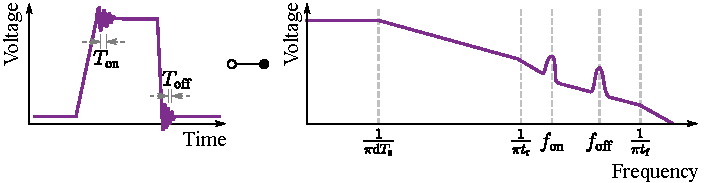
\includegraphics[scale = 1]{figures/2_Fundamentals/Diss_SpectrumCreation_res.pdf}
	\caption{Graphical representation of the creation of the emission spectrum from a resonant approximation of the switching transient.}
	\label{fig:Diss_SpectrumCreation_res}
\end{figure}

Taken together, the transition and resonance models explain individual features of the spectrum without reproducing the complete switching process.
Voltage-dependent capacitances and interactions between the gate and power circuits further modify the waveform, limiting the quantitative accuracy of these idealized representations.

\subsubsection*{Gaussian Smoothing as a Theoretical Reference}
Transition duration alone does not determine high-frequency emissions; waveform smoothness also affects spectral decay. 
Piecewise-linear transitions have discontinuities in their first derivatives, giving a high-frequency spectrum that decays in proportion to \SI{-40}{dB/dec}.
For comparison, convolution with a Gaussian kernel produces an infinitely differentiable ($C^\infty$) waveform, which can be expressed as:
\begin{equation}
	s(t) = \mi{V}{DC} \cdot \text{rect}\left(\frac{t}{\text{d}\mi{T}{s}}\right) * \left(\frac{1}{\sqrt{2\pi}\sigma_t}e^{-\frac{t^2}{2\sigma_t^2}}\right),
\end{equation}
where $\sigma_t$ is the standard deviation of the smoothing kernel.
Its Fourier transform yields
\begin{equation}
	S(f) = \mi{V}{DC} \cdot \text{d}\mi{T}{s} \cdot \text{si}(\pi f\text{d}\mi{T}{s}) \cdot e^{-(2\pi\sigma_t f)^2}.
\end{equation}
The Gaussian factor causes increasingly strong attenuation as frequency rises, so its envelope curves downward on a logarithmic-frequency plot instead of following a constant dB/decade slope, as illustrated in \fref{fig:Diss_SpectrumCreation_Heisenberg}:
For RMS measures of temporal and spectral width, the Gaussian kernel minimizes their product (the Heisenberg-Gabor limit) and thus provides a theoretical reference for minimizing spectral spread at a given temporal spread~\cite{signal_theory}.
Patin introduced this Gaussian waveform as the EM-noise-optimal switching waveform~\cite{Patin_HeisenbergGabor}.
In a power device, however, such a smooth, extended transition would be critical, since it prolongs the interval during which high voltage and high current are both present in the device, raising switching losses drastically.
The Gaussian waveform is therefore a theoretical benchmark; practical designs must balance spectral attenuation against switching loss.

\begin{figure}[h]
	\centering
	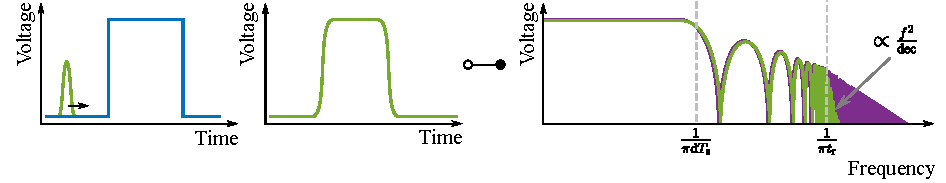
\includegraphics[scale = 1]{figures/2_Fundamentals/Diss_SpectrumCreation_Heisenberg.pdf}
	\caption{Graphical representation of the creation of the emission spectrum from a Gaussian approximation of the switching transient.}
	\label{fig:Diss_SpectrumCreation_Heisenberg}
\end{figure}

\subsubsection*{Simulated Spectra and the Need for Measurement}
\fref{fig:IntroFullSpec} shows the PSpice-simulated drain-source voltage of a hard-switched \SI{1200}{\volt} SiC MOSFET and its spectrum. Unlike the graphical approximations, the nonlinear device model captures switching transitions and circuit interactions, allowing comparison of the predicted envelope with the simulated spectrum.

\begin{figure}[ht]
	\begin{subfigure}{\textwidth}
		\centering
		\input{"figures/2_Fundamentals/DPT_TD_intro.tex"}
		\caption{PSpice-simulated drain-source voltage of a hard-switched SiC MOSFET.}
	\end{subfigure} %
	\par % Line break to stack subfigures
	\vspace{0.5cm}
	\begin{subfigure}{\textwidth}
		\hspace{-0.5cm}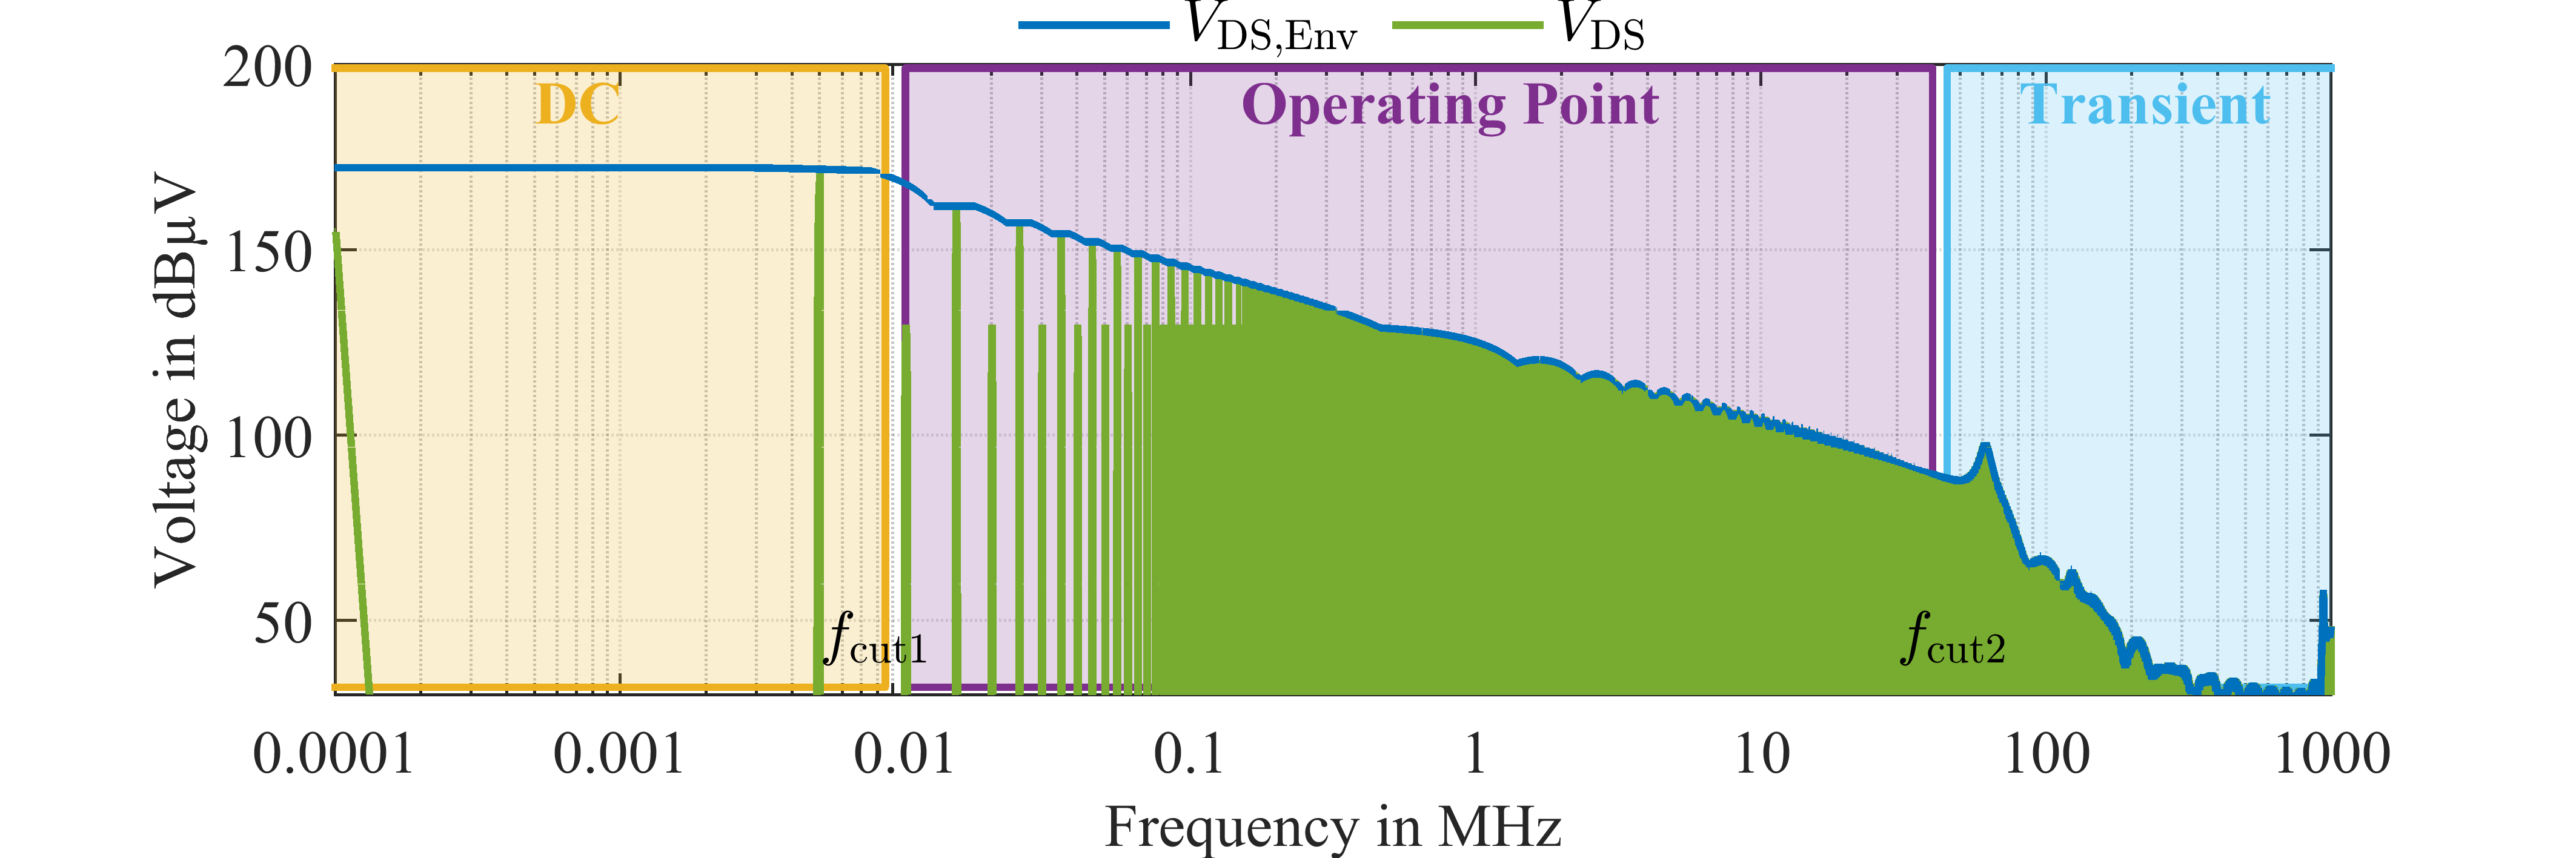
\includegraphics[scale = 1]{figures/2_Fundamentals/DPT_FD_intro.png}
		\caption{FFT of the simulated switching transient showing frequency regions dominated by different waveform phases.}
	\end{subfigure}
	\caption{Time-domain switching waveform and corresponding simulated voltage spectrum.}\label{fig:IntroFullSpec}
\end{figure}

Comparing the simulated spectrum with the graphical approximations shows that the rectangular-pulse model captures the low-frequency level and the approximately \SI{-20}{dB/dec} region. At higher frequencies, the spectrum departs from their constant-slope predictions as switching-edge details and circuit interactions become significant.

The regions labeled ``DC'', ``Operating Point'', and ``Transient'' in \fref{fig:IntroFullSpec} identify the dominant influences on different parts of the spectrum. 
The ``DC'' region is the low-frequency plateau, set by the DC-link voltage and duty cycle. In the ``Operating Point'' region, the switching frequency, duty cycle, and modulation strategy influence the spectrum. 
In the ``Transient'' region, the switching-edge duration and shape, together with associated oscillations, make the gate drive, device characteristics, and circuit parasitics important. 

\textbf{Limits of the Prediction:}
A physically plausible time-domain waveform does not establish the accuracy of its high-frequency spectrum, particularly above the dominant switching resonance.
The first limitation concerns model validation: calibration against conventional double-pulse measurements does not validate spectral components below the measurement noise floor, as discussed in the upcoming Section~\ref{sec:MeasurementLimitation}.
Agreement in switching time and overshoot can therefore coexist with substantial errors in much smaller high-frequency components.
The second limitation concerns numerical processing: solver tolerances, time steps and resampling all affect the computed spectrum.
Piecewise-linear interpolation, for example, can introduce derivative discontinuities and an artificial high-frequency tail.
The peak near \SI{900}{MHz} in \fref{fig:IntroFullSpec} illustrates the need to distinguish physical effects from numerical artifacts.
No physical mechanism could be identified to explain this peak, and it could be altered by changing the solver settings, indicating a numerical rather than a physical origin.
\\
\\
The graphical models provide a basis for interpreting the source spectrum, and simulation combines the underlying mechanisms within a circuit model.
Establishing the accuracy of the resulting predictions nevertheless requires measurements with sufficient bandwidth and dynamic range to resolve the relevant spectral components.
In the absence of a suitable measurement environment, none of the models considered here has yet been experimentally validated for predicting these small high-frequency spectral components.
Providing this experimental basis for model validation and the subsequent optimization of power-semiconductor switching behavior is a central aim of this thesis.

\FloatBarrier
\subsection{Propagation Paths in a Generic Inverter Application}
The switching transients discussed above excite noise currents that propagate through the inverter and its connected components to the external system ports.
The resulting conducted emissions depend on both the semiconductor switching behavior and the impedances of these propagation paths.
Although filtering and careful layout can reduce the coupling to external systems, complete suppression over the entire frequency range is not practically achievable.
% Characterizing the noise source therefore remains essential for understanding and mitigating system-level emissions.

\fref{fig:ESB_CMDM_Propagation} shows a simplified equivalent circuit for one phase of a three-phase machine inverter.
The circuit comprises an inverter half-bridge, the DC supply cables, and a machine represented by its winding impedance, the back electromotive force induced by rotor rotation, and parasitic capacitances to ground.
In an electric vehicle, this ground reference typically corresponds to the chassis rather than either DC supply conductor.
A line impedance stabilization network (LISN) is inserted between the power supply and the inverter to establish a defined impedance within the specified measurement band and to attenuate disturbances from the supply.
In the illustrated equivalent circuit, the LISN is represented by a $\pi$-type filter with a series inductor and shunt capacitive branches.
The inverter-side series $RC$ branch forms part of the low-impedance path for high-frequency disturbances. 
The measurement port is incorporated into this path, and the voltage across its termination resistance is measured.
This voltage is related to the noise current through the LISN transfer impedance; it is not a direct measurement of the total chassis current.

\begin{figure}[h]
	\centering
	\import{./figures/2_Fundamentals/}{Diss_ESB_CMDM_Propagation.pdf_tex}
	\caption{Equivalent circuit of the common-mode and differential-mode noise propagation paths.}
	\label{fig:ESB_CMDM_Propagation}
\end{figure}

The conducted noise currents at the LISN ports can be decomposed into differential-mode (DM) and common-mode (CM) components.
DM currents flow in opposite directions in the two supply conductors and close their loop through the power circuit.
CM currents, by contrast, flow in the same direction in both supply conductors and therefore require a ground return path. 


For the modal decomposition, \mi{I}{LISNp} and \mi{I}{LISNn} denote the noise currents in the positive and negative supply conductors at the LISN interface, respectively. 
The DM and CM components are then defined as
\begin{equation}
	\mi{I}{DM} = \frac{\mi{I}{LISNp} - \mi{I}{LISNn}}{2}
\end{equation}
and
\begin{equation}
	\mi{I}{CM} = \frac{\mi{I}{LISNp} + \mi{I}{LISNn}}{2}.
\end{equation}
With this convention, \mi{I}{CM} is the common-mode component per conductor.
Because the decomposition involves adding and subtracting the two currents, their relative timing or phase must be retained.
The equations therefore apply to instantaneous currents or complex frequency-domain quantities, not two independently measured spectral magnitudes.


Differential-mode currents are high-frequency components superimposed on the load current.
As the semiconductor devices switch, they draw pulsed current from the DC link.
The finite impedance of the DC-link capacitor allows this current to produce voltage fluctuations across the capacitor, which in turn drive the differential-mode current flowing in the supply conductors.

Switching transitions also excite common-mode currents, which flow through parasitic capacitances between circuit nodes and the chassis.
The parasitic capacitances \mi{C}{DC+} and \mi{C}{DC-} couple the positive and negative DC rails to ground, while \mi{C}{SwN} and \mi{C}{SP} represent the ground coupling of the switching node and the machine star point, respectively.
Changes in the voltage across these capacitances drive displacement currents according to $i_C = C\,\sddt{v}$.
These currents must return to their sources through the lowest-impedance path.
In an unfiltered setup, the return path may run through the chassis, the LISN, and the supply cables back to the inverter.
Y-capacitors, DC filters, and the design of the power cables can be used to shape this path in applications.

Which common-mode coupling path dominates depends strongly on the application.
The switching node experiences the highest voltage slew rate and is directly coupled to the chassis through \mi{C}{SwN}.
Although this capacitance is typically much smaller than the star-point capacitance, the high \sddt{v} can still produce a substantial displacement current.
The star-point capacitance is typically larger, but the voltage slew at the star point is reduced by capacitive voltage division across the motor winding capacitances.
Consequently, the larger capacitance does not necessarily produce a larger common-mode current.

The contributions of \mi{C}{DC+} and \mi{C}{DC-} to the common-mode current also depend on the commutation-loop design.
For example, when the DC rails have equal impedances and equal parasitic capacitances, their voltages vary in opposite directions relative to ground, causing the resulting ground-current contributions to cancel.
In coplanar designs, the parasitic capacitances of the two DC rails can be strongly asymmetric, increasing their net contribution to the common-mode current.
However, coplanar layouts also shield the switching node, reducing its coupling to the chassis and the contribution of \mi{C}{SwN}.
Overall, this shielding results in lower common-mode emissions in coplanar designs.

In addition to conducted emissions, the commutation loop also produces radiated emissions: its fast changing voltages and currents generate electric and magnetic fields that propagate through space.
Because no enclosure provides perfect shielding, some of these fields can escape through apertures and connectors.
Radiated emissions are particularly relevant above \SI{108}{\mega\hertz} and are typically measured in a shielded EMC chamber.

Because propagation paths strongly influence both conducted and radiated emissions, considerable research has addressed their characterization and mitigation.
This thesis, however, focuses on noise generation rather than on propagation and mitigation strategies.

\subsection{From Switching Sources to System-Level Emissions}


\begin{figure}
	\begin{subfigure}[t]{0.48\textwidth}
		\centering
		\raisebox{7mm}{\import{./figures/}{1_Introduction/NoiseGenerationSystem/DPT_TD.tex}}
		\subcaption{Drain-source voltages of the active and passive devices.}
		\label{fig:SourceToSystem_TD}
	\end{subfigure}
	\hfill
    \begin{subfigure}[t]{0.48\textwidth}
		\centering
		% \import{./figures/}{Snap_n_Mirror_vertical_v3_tex.pdf_tex}
		\import{./figures/}{GenerationVSpropagation_Converter.pdf_tex}
		\subcaption{Simplified equivalent circuit of the half-bridge converter.}
		\label{fig:SourceToSystem_Circuit}
	\end{subfigure}

	\vspace{0.5cm}
	\begin{subfigure}[t]{0.48\textwidth}
		\centering
		\import{./figures/}{1_Introduction/NoiseGenerationSystem/DPT_FD.tex}
		\subcaption{Voltage spectra of the active and passive devices.}
		\label{fig:SourceToSystem_Spectra}
	\end{subfigure}
	\hfill
	\begin{subfigure}[t]{0.48\textwidth}
		\centering
		\import{./figures/}{1_Introduction/NoiseGenerationSystem/TF_FD.tex}
		\subcaption{Artificial transfer functions from the devices to the LISN measurement port.}
		\label{fig:SourceToSystem_Transfer}
	\end{subfigure}
    
	\vspace{0.5cm}
    \begin{subfigure}[t]{0.98\textwidth}
		\centering
		\import{./figures/}{1_Introduction/NoiseGenerationSystem/System_FD.tex}
		\subcaption{Individual contributions and total LISN voltage spectrum with a emission limit. The limit is hypothetical and does not represent a CISPR compliance assessment.}
		\label{fig:SourceToSystem_LISN}
	\end{subfigure}
	\caption{Illustration of how switching noise sources and their propagation paths combine to shape the system-level emissions of a half-bridge converter, using simulated waveforms and artificial transfer functions.}
	\label{fig:SourceToSystem}
\end{figure}

The preceding subsections considered the generation and propagation of electromagnetic disturbances separately.
\fref{fig:SourceToSystem} combines these two aspects to illustrate how the switching waveforms of a half-bridge converter contribute to the voltage spectrum at a LISN measurement port.
The example uses simulated switching waveforms and artificial transfer functions to demonstrate the interaction between the noise sources and their propagation paths, rather than to predict the emissions of a specific prototype.



\fref{fig:SourceToSystem_TD} shows the drain-source voltages of the actively switched device and the complementary, passively commutated device.
Their different transition shapes and oscillations produce the source spectra shown in \fref{fig:SourceToSystem_Spectra}.
These spectra describe the disturbances at the devices, but do not directly indicate their contributions at the LISN measurement port.
As illustrated by the equivalent circuit in \fref{fig:SourceToSystem_Circuit}, each source is coupled to the measurement port through a different path.

The corresponding transfer functions in \fref{fig:SourceToSystem_Transfer} describe how strongly each frequency component is transmitted to the LISN measurement port.
Multiplying each complex source spectrum by its transfer function gives its contribution to the port voltage.
The total voltage is then obtained by adding these contributions with their relative phase retained.


\fref{fig:SourceToSystem_LISN} shows the individual contributions and the resulting LISN voltage spectrum.
The frequency dependence of the propagation paths changes the relative importance of the two sources and introduces spectral peaks and attenuation.
Consequently, a prominent feature at the measurement port need not correspond to a prominent feature in either source spectrum alone.
Reducing system-level emissions therefore requires considering both the switching behavior and the paths through which its disturbances propagate.
Whether the resulting emissions are acceptable is assessed using standardized measurement procedures and limits, introduced in the following subsection.

\FloatBarrier

\subsection{Standardized EMC Measurements and Limits}
Standardized emission measurements provide reproducible conditions for assessing the disturbances generated by a device under test (DUT).
CISPR, the International Special Committee on Radio Interference within the International Electrotechnical Commission (IEC), develops standards for such measurements and their limits.
For automotive applications, CISPR~25 specifies methods and limits for conducted and radiated disturbances.
The CISPR~16 series provides basic specifications for measuring apparatus and measurement methods, which are referenced where applicable by product standards.

Conducted emission measurements assess disturbances coupled into the connected wiring.
In the voltage method, a LISN establishes a defined supply impedance and couples the disturbance voltage to a measurement receiver.
Radiated emission measurements instead use antennas to measure the electromagnetic field produced by the DUT and its wiring under specified test conditions.
The antenna type, position, and polarization, together with the arrangement of the DUT and cables, are prescribed to obtain reproducible results.

In many EMC test schemes, conducted emissions are assessed up to \SI{30}{\mega\hertz}, while radiated measurements cover higher frequencies into the gigahertz range.
This division is not universal: the applicable frequency ranges depend on the product standard and measurement method, and automotive conducted-emission tests can extend beyond \SI{30}{\mega\hertz}.

Automotive inverter and converter suppliers may also be required to meet customer-specific conducted-emission limits up to \SI{100}{\mega\hertz} or higher.
Such requirements can supplement standardized tests with additional frequency ranges or stricter limits defined by the vehicle manufacturer rather than by the standard itself.
Their purpose is to reduce interference risks during component integration and to provide margin for the final vehicle-level EMC assessment.
Compliance at component level therefore supports, but does not guarantee, compliance of the complete vehicle, whose emission behavior also depends on the installed wiring and interactions between components.

The measured levels are compared with frequency-dependent limits for the applicable test method and limit class.
These limits must be used together with the specified receiver bandwidth and detector, such as peak, quasi-peak, or average, as applicable.
A simulated FFT spectrum cannot therefore be compared directly with a compliance limit unless the measurement conditions and receiver response are represented consistently.
The hypothetical limit in \fref{fig:SourceToSystem_LISN} is a simplification and is not taken from a standard: the figure shows the total LISN voltage \mi{V}{LISN}, whereas conducted-emission limits are specified separately for DM and CM measurements.

%!TeX root = main.tex
%!encoding = UTF-8 Unicode
\section{Dynamic Measurements for Power Electronics}

Dynamic characterization of power semiconductor devices is commonly performed in a half-bridge, where the devices are exposed to fast voltage and current transitions. 
Measuring these transients is challenging because the measurement system is connected directly to the circuit under test: it can alter the switching behavior, and its finite or non-ideal response can make the recorded waveforms differ from the actual device voltages and currents. 
The resulting errors arise from probe loading and circuit interaction, limited small-signal bandwidth, large-signal nonlinearities, parasitic capacitive and inductive coupling, transmission-line effects, and insufficient common-mode rejection. 
These mechanisms are illustrated in \fref{fig:ESB_MeasurementError} and are treated individually below. Establishing them as verification criteria is essential for assessing whether the measurement probes provide reliable measurements under the electrical and dynamic conditions of the half-bridge.
This discussion is directly relevant to this thesis, which develops a dual-channel differential active voltage probe and an active current shunt for measuring switching transients. 
The error mechanisms therefore provide the basis for defining the probes' design requirements and verification tests. 
Understanding them is also necessary to distinguish measurement-system artifacts from the actual behavior of the power semiconductor devices and to make reliable conclusions from the measured waveforms.

The figure shows the measurement of a high-side voltage and low-side current shunt measurement in a half-bridge including the different parasitics, couplings and effect which can alter the true device voltages and currents.
Here, the truth device voltages and currents are presented by the voltage applied directly at the power terminals of the devices, however these can never be measured directly for verification.

\begin{figure}
	\centering\import{./figures/2_Fundamentals/}{Diss_ESB_MeasurementErrors.pdf_tex}
	\caption{Circuit diagram of different sources of measurement error in a half-bridge circuit.}
	\label{fig:ESB_MeasurementError}
\end{figure}

\subsubsection*{Probe Loading and Circuit Interaction}
Any measurement sensor presents a finite impedance to the circuit under test and can therefore alter the quantity being measured. 
A voltage probe is connected in parallel with the circuit and should have a high input impedance, whereas a current sensor is inserted in series and should add as little impedance as possible.

For drain-source voltage measurements, the input capacitance of the probe is connected in parallel with the device output capacitance. 
Since the latter is typically on the order of hundreds of picofarads, it can reduce the relative influence of the probe capacitance. 
This does not eliminate loading, but it generally makes input capacitance less restrictive than it would be in a measurement with a much smaller load capacitance, as for example the measurement of the switching-node in relation to GND.

\begin{figure}[h]
	\centering
	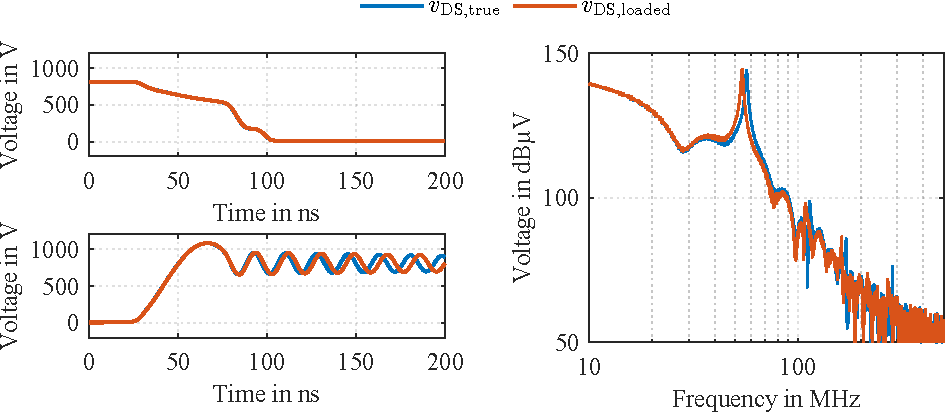
\includegraphics[scale = 1]{figures/2_Fundamentals/MeasurementErrors_Plots/Fundamental_Loading_TDFD.pdf}
	\caption{Simulation results of capacitive loading with $\mi{C}{probe} = 0.1 \mi{C}{oss}(\SI{800}{V})$.}
	\label{fig:Fundamental_Loading_TDFD}
\end{figure}
  
% Streit_ECCE_Asia
                  
Current measurement in the commutation loop presents a different challenge. 
The loop inductance is deliberately minimized because it contributes to switching overvoltage and losses, and can be only a few nanohenries. 
The parasitic inductance introduced by a series current shunt may therefore be comparable to the loop inductance itself and perturb the current transient being measured.

The significance of a sensor's ohmic resistance also depends on the measurement objective. 
In conventional switching characterization, its effect may be secondary to that of parasitic inductance. In EMC-relevant measurements, however, the shunt resistance can affect the measured current and the circuit under test; this issue is discussed further in Chapter~\ref{ch:AShunt}.

As a practical loading criterion, the input impedance of a voltage probe should be at least one decade greater than the impedance of the measured source. 
Conversely, the series impedance of a current sensor should be at least one decade lower than the impedance of the circuit into which it is inserted. 
These criteria limit, but do not by themselves eliminate, measurement-induced changes to the circuit.

\subsubsection*{Small-Signal Response and Bandwidth Criteria}
The small-signal response describes how a measurement probe transfers input signals over frequency when operated within its linear range. 
It is commonly represented by the transfer function, whose magnitude determines the frequency-dependent gain and whose phase describes the relative phase shift between the input and output. 
Although switching transients are large-signal events in the time domain, their shape contains frequency components across a broad range. 
Consequently, the probe's small-signal frequency response provides a first measure of whether those components are reproduced faithfully.

If the probe bandwidth is insufficient, higher-frequency components are attenuated, which can make measured edges appear slower and can suppress high-frequency ringing. 
Gain variation within the frequency range of interest can likewise alter the relative amplitudes of spectral components. 
Frequency-dependent phase shift can further change the reconstructed waveform. Thus, a probe may produce a plausible waveform while still misrepresenting the amplitude or timing of fast features.

\begin{figure}[h]
	\centering
	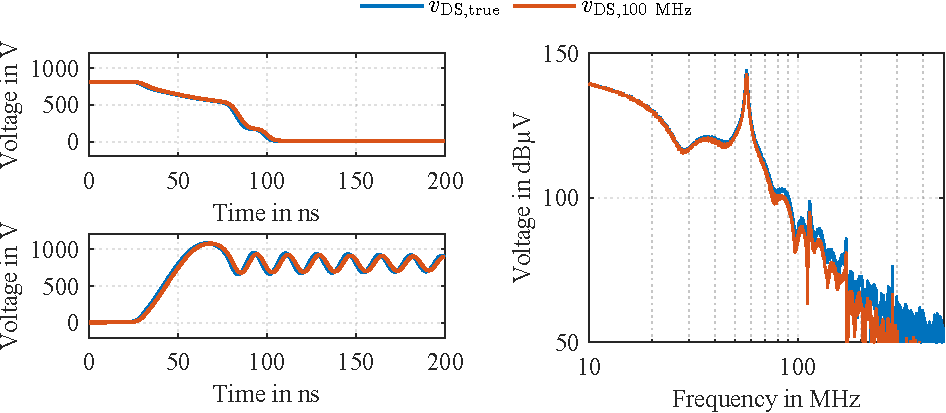
\includegraphics[scale = 1]{figures/2_Fundamentals/MeasurementErrors_Plots/Fundamental_100MHz_TDFD.pdf}
	\caption{Simulation results of probe small-signal frequency response with $\mi{f}{probe} =\SI{100}{MHz}$.}
	\label{fig:Fundamental_Loading_TDFD}
\end{figure}



The bandwidth requirement should be related to the maximum frequency of interest in the measurement, rather than to the fastest frequency the instrument can display. 
A common criterion is that the probe's $-3$\,dB bandwidth exceed this maximum frequency. 
This criterion places the frequency of interest below the point at which the response magnitude has fallen to approximately $0.707$ of its reference value; it does not, by itself, guarantee flat gain or negligible phase distortion throughout the band. 

Small-signal frequency response is typically characterized with a vector network analyzer (VNA), which measures the probe's transfer response under a low-level sinusoidal excitation over a swept frequency range. 
The resulting magnitude response can be used to evaluate gain flatness and bandwidth. 
This test characterizes linear frequency-dependent behavior; it does not establish that the probe remains linear under large input amplitudes, which must be assessed separately.

\subsubsection*{Large-Signal Response and Nonlinearities}

Small-signal characterization does not establish that a probe remains accurate at the amplitudes encountered in operation. 
VNA measurements are typically performed with millivolt-level excitation, well below the signal levels experienced by the sensor during normal use. 
Active sensors may become nonlinear as their input or output stages approach voltage or current limits; finite slew rate and overload recovery can also distort fast transitions. 
Magnetic sensors may additionally exhibit hysteresis or saturation, making their response dependent on signal amplitude and, in the case of hysteresis, on their prior magnetic state. 
These effects can cause gain compression, clipping, altered edge shapes, or delayed settling and cannot be inferred from a low-level frequency-response measurement.

Large-signal verification therefore requires excitation representative of both the intended signal amplitude and transient speed, together with an independent reference measurement. 
Such a test can reveal gain compression, clipping, hysteresis, and overload recovery. 
Its conclusions apply only to the amplitudes and transient speeds tested.
In practice, producing a representative signal and obtaining a reliable reference measurement are often the main challenges.


\subsubsection*{Parasitic Coupling Paths}
Parasitic coupling provides unintended paths for switching transients to enter a sensor without passing through its intended sensing element. In a half-bridge, fast voltage transitions drive displacement currents through stray capacitances, while rapidly changing commutation-loop currents induce voltages through mutual inductance. In \fref{fig:ESB_MeasurementError}, these paths are modeled by the parasitic capacitances \mi{C}{\sigma+} and \mi{C}{\sigma-} and the mutual inductances \mi{L}{\mathrm{m,i}} and \mi{L}{\mathrm{m,v}}. Coupling strength depends on the circuit layout and sensor placement, and generally increases with the rate of voltage or current change.

For the current-sensing arrangement in \fref{fig:ESB_MeasurementError}, the measured sense voltage can be written as the sum of the desired shunt voltage and the coupled contributions:
\begin{equation}
    \mi{v}{sense} = \mi{R}{shunt} \mi{i}{S} - \mi{L}{\mathrm{m,i}} \ddt{\mi{i}{S}} - \mi{R}{shunt}\mi{C}{\sigma}  \ddt{\mi{v}{DS}}
    \label{eq:parasitic_coupling_current_sense}
\end{equation}
assuming an ohmic shunt and the reference directions shown in the figure. 
The second term represents inductive pickup from the changing current. 
The final term represents capacitive feedthrough from the drain-source voltage; it is proportional to the imbalance between the two coupling capacitances. 
Thus, matched capacitances cancel in this model, whereas any mismatch converts part of the voltage slew rate into an apparent shunt voltage.

\begin{figure}[h]
	\centering
	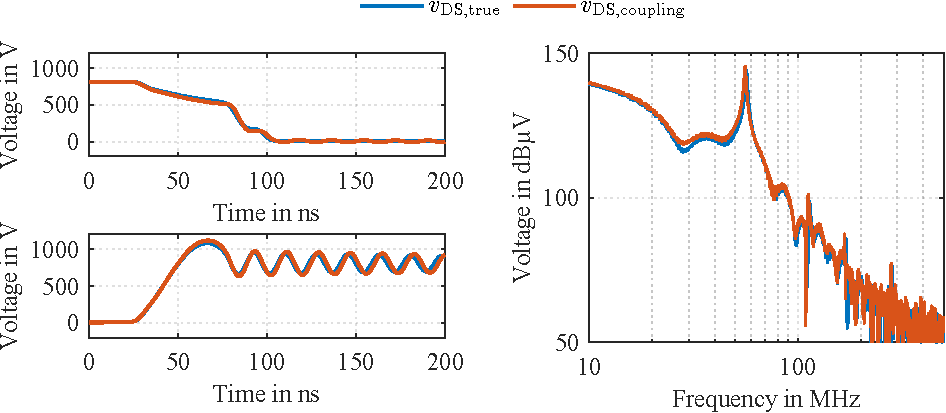
\includegraphics[scale = 1]{figures/2_Fundamentals/MeasurementErrors_Plots/Fundamental_Coupling1n_TDFD.pdf}
	\caption{Simulation results of inductive coupling with \SI{1}{nH} and a coupling factor of 1.}
	\label{fig:Fundamental_Coupling_TDFD}
\end{figure}

The coupling error can be difficult to identify from the waveform alone. 
Both the desired current and the parasitic contributions are driven by the same switching event, so the measured signal may remain synchronized with the expected current waveform and appear plausible. Nevertheless, the coupled terms can change its amplitude and spectral content, or produce transient features that are incorrectly attributed to the device under test. 
Detection therefore requires comparison with an independent reference. 
Sensitivity can also be assessed by changing sensor position, orientation, or shielding while holding the circuit conditions constant; a resulting change in the measurement indicates susceptibility to parasitic coupling.

\subsubsection*{Transmission-Line Effects}
Measurement cables possess distributed resistance, inductance, and capacitance. Once the cable length is no longer negligible compared with the wavelength of the signal components of interest, it must be treated as a transmission line rather than as an ideal connection. The signal then propagates along the cable at the velocity
\begin{equation}
    \mi{c}{W} = \frac{1}{\sqrt{\mi{L}{W}\mi{C}{W}}},
    \qquad
    \mi{Z}{W} = \sqrt{\frac{\mi{L}{W}}{\mi{C}{W}}},
    \qquad
    \lambda = \frac{\mi{c}{W}}{f},
\end{equation}
where \mi{L}{W} and \mi{C}{W} denote the cable's inductance and capacitance per unit length, \mi{Z}{W} is its characteristic impedance, and \mi{c}{W} is its propagation velocity. A cable of length $l$ thus introduces a one-way propagation delay $\tau = l/\mi{c}{W}$.

At each cable termination, any mismatch between the termination impedance and \mi{Z}{W} causes part of the incident voltage wave to be reflected. The voltage reflection coefficient at termination $k$ is
\begin{equation}
    \mi{\Gamma}{k}(t) = \frac{\mi{Z}{k}(t) - \mi{Z}{W}}{\mi{Z}{k}(t) + \mi{Z}{W}},
    \qquad k \in \{L,Q\},
\end{equation}
where \mi{Z}{L} is the load impedance and \mi{Z}{Q} is the effective MOSFET impedance seen by the cable, as shown in \fref{fig:TransmissionLineMeasurementCable}. In a drain-source voltage measurement, \mi{Z}{Q} changes as the MOSFET switches between its off-state, transition, and on-state conditions, so the source-side reflection coefficient varies throughout the switching event. If either termination is mismatched, the reflected wave travels back along the cable and may be reflected again at the opposite end. These repeated reflections can produce overshoot, ringing, and delayed settling, distorting the amplitude and shape of fast transitions; this effect becomes significant once the propagation delay is comparable with the transition time.

\begin{figure}
	\centering\import{./figures/2_Fundamentals/}{SourceImpedanceMOSFET_cable.pdf_tex}
	\caption{Equivalent circuit illustrating cable reflections and the time-varying MOSFET impedance in a drain-source voltage measurement.}
	\label{fig:TransmissionLineMeasurementCable}
\end{figure}

Impedance matching, typically achieved by terminating the cable in its characteristic impedance, minimizes these reflections. When matching is not applied, the cable should instead be kept electrically short over the frequency range of interest. A common criterion is
\begin{equation}
    l < \frac{\lambda_{\min}}{10} = \frac{\mi{c}{W}}{10 f_{\max}},
\end{equation}
where $f_{\max}$ is the highest frequency component that must be measured faithfully and $\lambda_{\min}$ is the corresponding wavelength in the cable. Under this condition, the cable can generally be approximated as a lumped interconnect, although the residual error still depends on the source and load impedances and on the required measurement accuracy. For fast switching transients, the relevant frequency range is set by the edge content of interest rather than by the switching repetition frequency alone.

\begin{figure}[h]
	\centering
	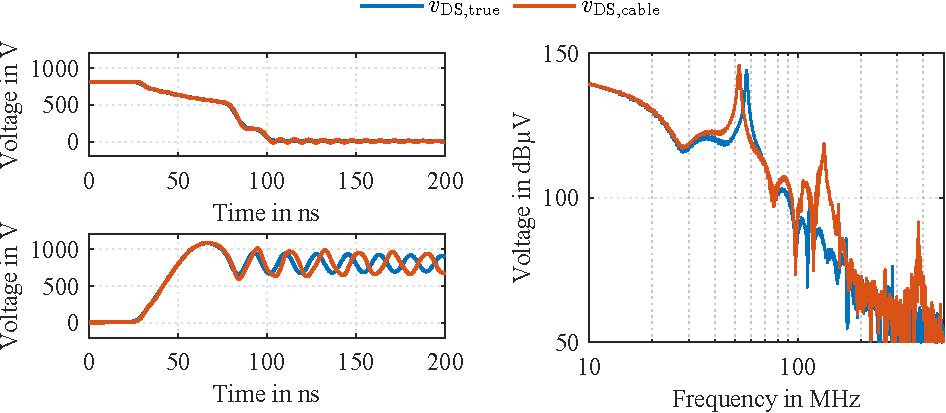
\includegraphics[scale = 1]{figures/2_Fundamentals/MeasurementErrors_Plots/Fundamental_cable_TDFD.pdf}
	\caption{Simulation results of voltage measurement with \SI{1}{m} and \SI{50}{\Omega} coaxial cable.}
	\label{fig:Fundamental_Cable_TDFD}
\end{figure}


\FloatBarrier

\subsubsection*{Common-Mode Rejection}
A measurement referenced to the oscilloscope ground adds any difference between its own local ground potential and the oscilloscope's ground potential directly onto the measured signal. 
This common-mode voltage \mi{v}{cm} is attenuated, but not eliminated, by the measurement system's common-mode rejection ratio,
\begin{equation}
    \mathrm{CMRR} = \frac{\mi{A}{diff}}{\mi{A}{cm}},
\end{equation}
defined as the ratio of the differential-mode gain \mi{A}{diff} to the common-mode gain \mi{A}{cm}. Referred to the input, the resulting measurement error is
\begin{equation}
    \mi{e}{cm} = \frac{\mi{v}{cm}}{\mathrm{CMRR}}.
\end{equation}

Common-mode rejection is most critical for the gate-source voltage measurement, since the gate driver's reference potential is tied to the switching MOSFET's source terminal, which itself swings with the switching-node voltage; the resulting common-mode voltage can become comparable to, or even exceed, the gate-source signal of interest. 
This measurement is not performed in this thesis.

For the drain-source voltage and current-shunt measurements treated here, the dominant common-mode disturbance instead arises from a ground bounce: the commutation-loop current \mi{i}{S} driven through the stray inductance \mi{L}{\sigma} of the common return path displaces the oscilloscope's local ground reference relative to the true circuit ground by
\begin{equation}
    \mi{v}{cm} \approx \mi{L}{\sigma}\ddt{\mi{i}{S}}.
\end{equation}
This ground bounce is not necessarily negligible, as the shunt signal itself can also be small. 
A sufficient criterion is that the common-mode error remain below the required measurement accuracy $e_{\max}$, that is
\begin{equation}
    \mathrm{CMRR} \geq \frac{\mi{v}{cm}}{e_{\max}} = \frac{\mi{L}{\sigma}\ddt{\mi{i}{S}}}{e_{\max}}.
\end{equation}


\subsubsection*{Summary of Measurement Errors and Verification Criteria}

Table \ref{tab:dynamic_measurements} summarizes the error mechanisms discussed above, together with a suitable verification test, the problem it reveals, and the resulting criterion. The criteria differ in character: loading, bandwidth, and large-signal behavior can be assessed from the probe's own specifications and a dedicated calibration measurement, whereas parasitic coupling and transmission-line effects depend on the specific setup and therefore require a comparative measurement against an independent reference.

\begin{table}[htbp]
\caption{Dynamic measurements and verification criteria}
\label{tab:dynamic_measurements}
{%
\renewcommand{\tabularxcolumn}[1]{m{#1}}
    \begin{tabularx}{\textwidth}{>{\raggedright\arraybackslash}X>{\raggedright\arraybackslash}X>{\raggedright\arraybackslash}X>{\raggedright\arraybackslash}X}
        \toprule
        \textbf{Test} & \textbf{Verification test} & \textbf{Problems} & \textbf{Verification} \\
        \midrule
        Loading & Impedance measurement & Influencing DUT operation & 1 decade higher/lower \\
        \midrule
        Small signal response & VNA measurements & - Bandwidth \newline - gain flatness & $f_{\text{3dB}} > f_{\text{interest,max}}$ \\
        \midrule
        Large signal response & Pulse generator & Nonlinearities: \newline - Saturation \newline - Hysteresis \newline - ... & $t_r > t_{\text{r,meas,min}}$ \\
        \midrule
        Parasitic coupling & Measurement in parallel to verified sensor in setup & - Capacitive coupling of voltage transient \newline - Inductive coupling of current transient & Matching with verifying sensor \\
        \midrule
        Transmission line & Measurement in parallel to verified sensor in setup & - Wave reflection \newline - Signal distortion & Matching with verifying sensor \\
        \bottomrule
    \end{tabularx}
}
\end{table}

No single test covers all mechanisms: a probe that passes the loading and bandwidth criteria can still be compromised by parasitic coupling or an unterminated cable, and vice versa. 
The criteria must therefore be verified individually, each with its own excitation and reference measurement, with thresholds adapted to the frequency and amplitude range relevant to the measurement task at hand. 
Only once all criteria are satisfied jointly can the subsequent measurements be treated as representative of the true device voltages and currents, rather than as artifacts of the measurement system itself.

% %!TeX root = main.tex
%!encoding = UTF-8 Unicode
\section{Noise-Induced Measurement Limitations}
\label{sec:MeasurementLimitation}

To motivate the dedicated measurement approach, this section analyzes the noise-induced limitations that arise when a switching voltage waveform is measured with a conventional probe and digitized by an oscilloscope ADC\@.
These limitations are particularly significant for small, high-frequency signal components relevant to EMC analysis.
For conventional switching metrics, such as overvoltage, $\sddt{v}_\text{max}$, and switching energy, their influence is typically negligible under the measurement conditions considered.

\fref{fig:QuantNoise} illustrates these limitations in the time and frequency domains by comparing a simulated voltage transient with its quantized counterpart contaminated by thermal noise.
The spectral plot focuses on \SIrange{10}{500}{MHz}, where switching transients are particularly relevant to the electromagnetic emission behavior of power semiconductor devices.
Electromagnetic emissions from inverters remain relevant above this range; however, practical experience from measurements in the EMC chamber indicates that emissions above approximately \SI{500}{MHz} are often dominated by digital clocking in microcontrollers or FPGAs rather than by power semiconductor switching.
This frequency therefore serves as an empirical guideline for the scope of the present analysis, not as a strict boundary between emission sources.


\subsection{Thermal Noise}

Thermal noise arises from the random thermal motion of charge carriers in every resistive element of the measurement system.
The RMS thermal noise voltage across a resistance can be expressed as
\begin{equation}
	\mi{v}{n,th,RMS} = \sqrt{4 k_B T R \Delta f},
\end{equation}
where $k_B$ is the Boltzmann constant, $T$ is the absolute temperature, $R$ is the resistance, and $\Delta f$ is the measurement bandwidth.
Its power spectral density is approximately constant over the frequency range considered, so its RMS amplitude increases with the square root of the measurement bandwidth.

For the following analysis, the differential probe and oscilloscope are taken as the dominant sources of measurement noise.
Thermal noise from the device under test is neglected by approximating its drain-source impedance as an ideal capacitance with zero equivalent series resistance.

In the oscilloscope, resistive elements in the input attenuator and amplifier stages generate thermal noise, while the active circuitry introduces additional electronic noise.
The measured RMS noise depends on the selected vertical range, which determines the input attenuation and amplification.

In the differential probe, the resistive voltage divider and amplifier circuitry likewise contribute noise.
A higher probe attenuation reduces the signal reaching the oscilloscope, making the oscilloscope noise more significant when referred back to the measured voltage.

For both instruments, the analogue bandwidth determines the integrated noise level.
Reducing this bandwidth lowers the RMS noise, but also suppresses high-frequency signal components.
Since the present analysis requires accurate measurement of signal components up to \SI{500}{MHz}, bandwidth reduction cannot be used to lower the noise floor at the expense of the required frequency response.
The noise specifications must therefore be evaluated for the selected vertical range and probe attenuation, with sufficient analogue bandwidth to preserve these components.

The following calculation uses the noise values specified in the instrument datasheets: \SI{1.61}{mV} for the oscilloscope at \SI{100}{mV/div} and \SI{500}{MHz} bandwidth~\cite{tektronix_mso_2026} and \SI{55}{mV} for the differential probe at an attenuation ratio of \mti{a}{probe}~=~250~\cite{pmk_gmbh_datasheet_2017}.
These specifications include electronic noise contributions beyond purely thermal noise and are used here to estimate the analogue measurement noise floor.
For this estimate, both values are interpreted as RMS voltages, with the probe noise referred to its output and the oscilloscope noise referred to its input.
Assuming uncorrelated noise sources and a frequency-independent probe attenuation over the range considered, their noise powers add.
The combined RMS noise referred to the high-voltage side is therefore

\begin{equation}
	\mi{V}{n,th,RMS} = \mti{a}{probe}\sqrt{\mi{v}{n,th,osci}^2 + \mi{v}{n,th,probe}^2}
	\approx \SI{13.76}{V}.
\end{equation}

The symbol \mi{V}{n,th,RMS} denotes the combined analogue noise estimate, including the additional electronic noise contained in the datasheet specifications.
To estimate its contribution to the spectral noise floor, each source is approximated as white noise over its equivalent noise bandwidth.
The RMS noise in an FFT bin, referred to the high-voltage side, is then

\begin{equation}
	\mi{V}{th,bin,RMS} = \mti{a}{probe}\sqrt{
	\left(\frac{\mi{v}{n,th,osci}^2}{\mi{B}{n,osci}}
	+ \frac{\mi{v}{n,th,probe}^2}{\mi{B}{n,probe}}\right)\mi{B}{bin}},
	\label{eq:RMStoAmplitudePlot}
\end{equation}

Here, \mi{B}{n,osci} and \mi{B}{n,probe} are the equivalent noise bandwidths associated with the respective RMS specifications, including any subsequent filtering in the measurement chain.
If filtering changes a source's bandwidth, its integrated RMS noise must also be adjusted consistently.
These bandwidths depend on the analogue frequency responses and are not generally equal to the Nyquist frequency.
The nominal \SI{500}{MHz} oscilloscope bandwidth is a signal-bandwidth specification and need not equal its equivalent noise bandwidth.

The quantity \mi{B}{bin} is the equivalent noise bandwidth of the FFT window: for a rectangular window, it equals the bin spacing $\Delta \mi{f}{bin} = \mi{f}{s}/\mi{N}{FFT}$, while other windows require a window-dependent correction.
The estimate represents RMS noise per bin; comparison with the plotted FFT requires consistent window and amplitude normalization.
In logarithmic form, the RMS bin noise becomes
\begin{equation}
	\mi{V}{th,bin,RMS}^{\mathrm{dB}\upmu\mathrm{V}} = 20 \cdot \log_{10}\left(\frac{\mi{V}{th,bin,RMS}}{\SI{1}{\micro V}}\right).
\end{equation}

This analogue noise floor can mask small high-frequency signal components even when the measurement system provides sufficient signal bandwidth.









\subsection{Quantization Noise}
\label{sec:QuantNoise}

In addition to analogue noise, digitization by the oscilloscope introduces quantization error.
The oscilloscope's ADC represents each sampled input voltage by one of a finite number of discrete amplitude levels.
The difference between the input voltage and the assigned level is the quantization error; for ideal rounding without clipping, its magnitude is bounded by half the quantization step.
For a given ADC resolution, a wider input voltage range increases the spacing between these levels.
The vertical range required to capture the full switching transient therefore affects the resolution available for its small high-frequency components.

Quantization error is inherently signal-dependent and may produce discrete spectral components when its pattern repeats. 
For the following noise-floor estimate, however, it is approximated as uniformly distributed between adjacent quantization levels and uncorrelated with both the input signal and errors at other sampling instants. 
Under these assumptions, it can be modeled as additive white quantization noise.

The quantization process can be written as a rounding function that maps the input signal to the nearest quantization level:
\begin{equation}
	Q(\mi{v}{DS}) = \text{round}\left(\frac{\mi{v}{DS}}{q}\right) \cdot q,
	\label{eq:quantization}
\end{equation}

Here, $q$ is the ADC quantization step, calculated as
\begin{equation}
	q = \dfrac{\mi{V}{max}-\mi{V}{min}}{2^{\mti{N}{ENOB}}}.
\end{equation}

The effective number of bits (ENOB) is typically lower than the nominal ADC resolution (\mi{N}{ADC}) because of non-idealities in the sampling process, such as jitter, thermal noise, and other error sources. It also decreases with frequency~\cite{tektronix_mso_2026}.

Assuming a uniform distribution of the quantization error, the quantization noise is calculated as
\begin{equation}
	\mi{V}{quant,RMS} = \sqrt{\frac{q^2}{12}}
\end{equation}
The derivation of this expression is omitted here and can be found in~\cite{silicon_laboratories_an118_2013}.

For an ideal ADC with white, uncorrelated quantization error, the quantization noise is distributed over the Nyquist bandwidth $\mi{f}{s}/2$.
Using the same RMS-per-bin normalization as in Eq.~\ref{eq:RMStoAmplitudePlot}, its spectral contribution is
\begin{equation}
	\mi{V}{quant,bin,RMS} = \mi{V}{quant,RMS}\sqrt{\frac{\mi{B}{bin}}{\mi{f}{s}/2}},
\end{equation}
where the noise and signal amplitudes must be referred to the same point in the measurement chain.









\subsection{Implications for  Measurements of Switching Transient}

The analogue and quantization noise contributions jointly limit the spectral information that can be extracted from a measured switching transient.
Under the assumption of uncorrelated analogue and quantization noise, their RMS contributions within the same FFT bin combine as
\begin{equation}
	\mi{V}{noise,bin,RMS} = \sqrt{\mi{V}{quant,bin,RMS}^2 + \mi{V}{th,bin,RMS}^2},
\end{equation}
with both contributions referred to the same point in the measurement chain.
The following simulation illustrates the resulting limitations for a conventional probe and oscilloscope measurement chain.

\begin{figure}[!htbp]
	\begin{subfigure}{\textwidth}
		\centering
		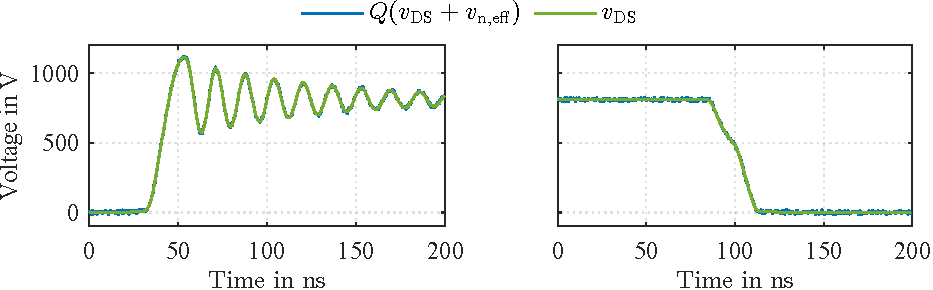
\includegraphics[scale = 1]{figures/3_Methods/Measurement_Limitation/DPT_TD_new.pdf}
		\caption{Simulated drain-source voltage switching transient in the time domain, with and without thermal and quantization noise (PSpice).}
	\end{subfigure}\par
	\vspace{1cm}\par
	\begin{subfigure}{\textwidth}
		\hspace{-0.7cm}
		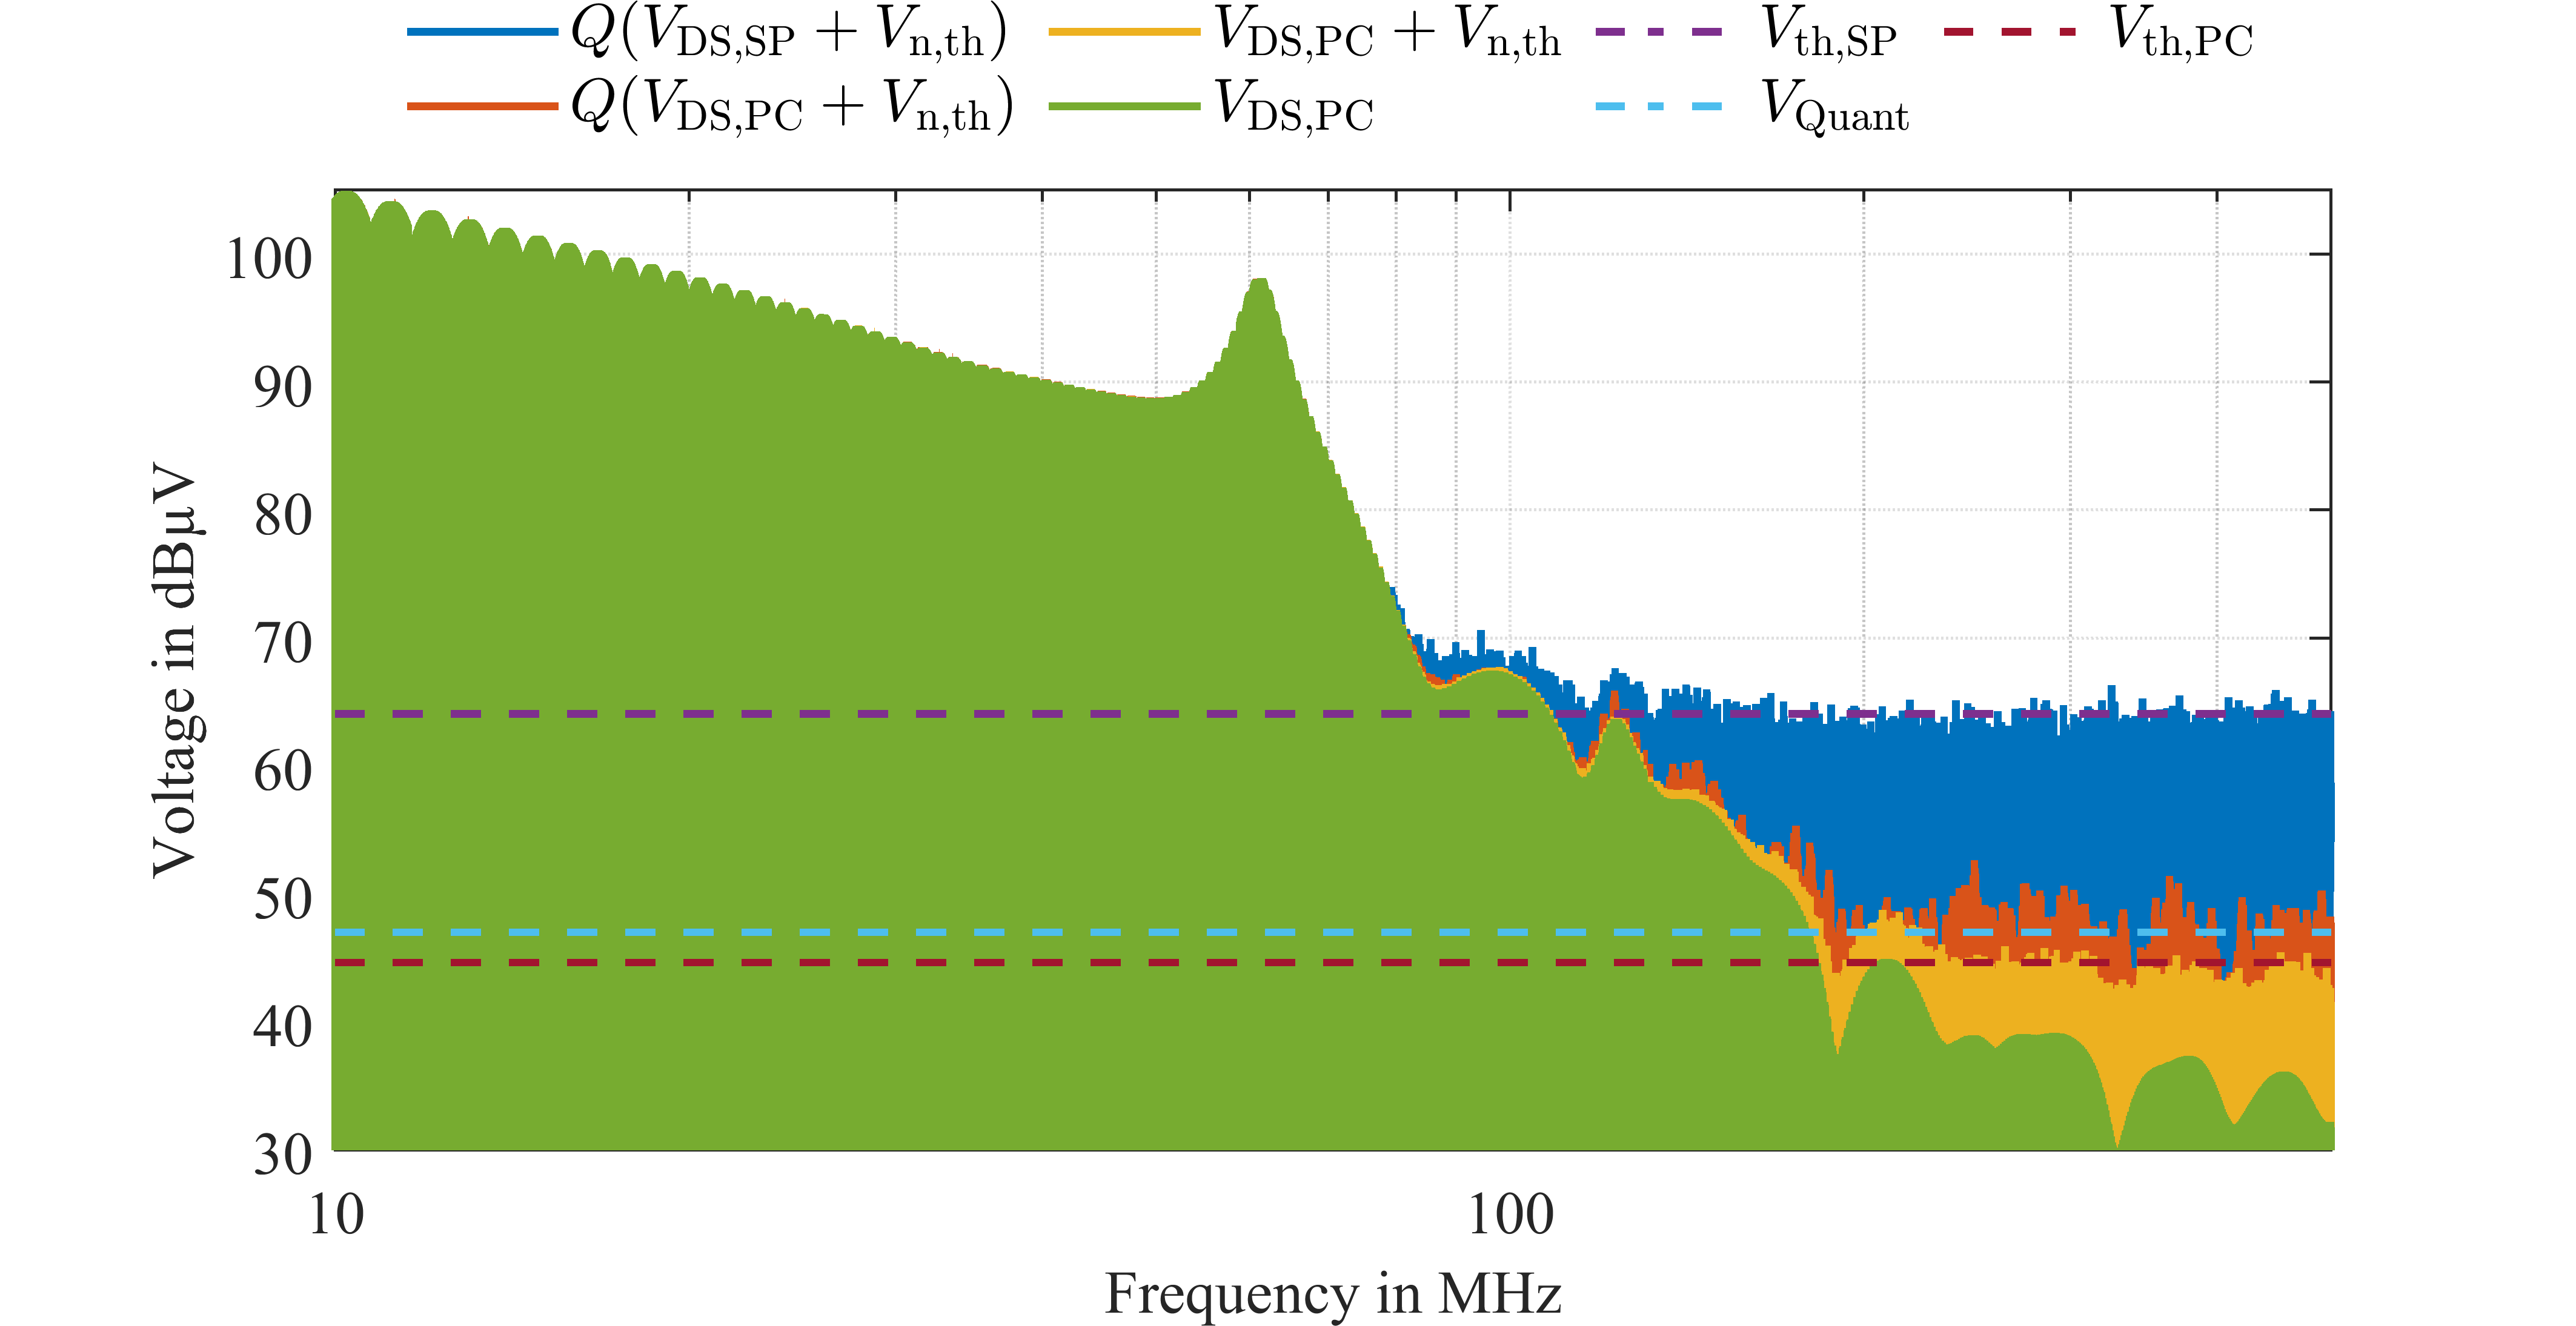
\includegraphics[scale = 1]{figures/3_Methods/Measurement_Limitation/DPT_FD_new.png}
		\caption{FFT of the simulated signal with and without thermal and quantization noise, shown for a single pulse (SP) and a pulse chain (PC). Calculated noise floors are added in dashed lines.}
	\end{subfigure}
	\caption{Noise-induced measurement limitations for switching transients in the time and frequency domains.}\label{fig:QuantNoise}
\end{figure}

Figure~\ref{fig:QuantNoise} compares the spectrum of the quantized, noise-contaminated single-pulse (SP) signal, $Q(\mi{V}{DS,SP}+\mi{V}{n,th})$, shown in blue, with that of the noise-free pulse-chain (PC) signal, $\mi{V}{DS,PC}$, shown in green.
The single-pulse signal represents a double-pulse test, which is commonly used to characterize power semiconductor devices.
The remaining spectra illustrate the effects of the measurement methods introduced in the following subsections to mitigate these noise limitations.

In the simulated single-pulse measurement, the signal spectrum falls below the noise floor at approximately \SI{80}{MHz}, above the resonance at \SI{62}{MHz}.
Beyond this frequency, the high-frequency voltage components cannot be reliably distinguished from measurement noise under the conditions considered.

The resonance is governed by the MOSFET output capacitance and commutation-loop inductance.
Typical resonance frequencies are approximately \SIrange{10}{50}{MHz} for modules and \SIrange{80}{120}{MHz} for discrete devices.

As discussed in Chapter~\ref{ch:Fundamentals}, finite switching transition times cause the high-frequency spectral envelope to decay, reducing the signal amplitudes available for measurement.
The noise-floor crossing therefore depends on both the signal spectrum and the measurement conditions; it is not fixed by the resonance frequency alone.

A numerical example illustrates the scale of these spectral amplitudes relative to an ENOB-based equivalent voltage step.
For unequal rise and fall times, the high-frequency spectral envelope can be estimated as~\cite{bi_prediction_2019}
\begin{equation}
	\mi{V}{DS,env}(f) = \dfrac{\mi{V}{DC}\mi{f}{sw}}{\uppi^2 f^2}
	\left(\dfrac{1}{\mi{\tau}{r}}+\dfrac{1}{\mi{\tau}{f}}\right),
	\quad f > \dfrac{1}{\uppi\min(\mi{\tau}{r},\mi{\tau}{f})}.
\end{equation}
With $\mi{V}{DC} = \SI{800}{V}$, $\mi{f}{sw} = \SI{25}{kHz}$, $\mi{\tau}{r} = \SI{20}{ns}$, and $\mi{\tau}{f} = \SI{50}{ns}$, the envelope at \SI{100}{MHz} is approximately \SI{14.2}{mV}.
For a probe attenuation of $\mti{a}{probe} = 250$, the corresponding envelope amplitude referred to the ADC input is
\begin{equation}
	\mi{v}{ADC,in} = \dfrac{\mi{V}{DS,env}(\SI{100}{MHz})}{\mti{a}{probe}}
	= \dfrac{\SI{14.2}{mV}}{250} \approx \SI{57}{\micro V}.
\end{equation}
For comparison, an assumed effective resolution of $\mti{N}{ENOB} = 14$ bits and an input range corresponding to \SI{-150}{V} to \SI{1200}{V} on the measured side yield an equivalent voltage step referred to the ADC input of
\begin{equation}
	\mi{q}{ADC,eff} = \dfrac{\mi{V}{max}-\mi{V}{min}}{\mti{a}{probe}\,2^{\mti{N}{ENOB}}}
	= \dfrac{\SI{1200}{V}-(\SI{-150}{V})}{250\cdot 2^{14}}
	\approx \SI{330}{\micro V}.
\end{equation}
The estimated signal amplitude is approximately six times smaller than the equivalent voltage step, placing both within one order of magnitude and illustrating the resolution challenge.

These small high-frequency voltage components are primarily relevant to EMC analysis.
Under the measurement conditions considered, their influence on conventional metrics such as overvoltage, switching energy, and $\sddt{v}_\text{max}$ is typically negligible.
Characterizing SiC MOSFETs over the EMC-relevant frequency range of \SIrange{10}{500}{MHz} therefore requires methods that reduce these noise limitations while preserving the required signal bandwidth.
The following subsections introduce the corresponding measurement methods.